\documentclass[11pt,a4j]{jarticle}%jarticleを使用
\usepackage[dvipdfmx]{graphicx}%画像表示の設定
\usepackage{amsmath}%数式周りの強化
\usepackage[all, warning]{onlyamsmath}%eqnarrayを禁止
\usepackage[top=5truemm,bottom=30truemm,left=20truemm,right=20truemm]{geometry}%ページの余白を調整
\usepackage{cite}%引用を整備
\usepackage{ascmac}%screen環境による箱囲みを利用
\usepackage{url}%urlを成形する
\usepackage{here}
\usepackage{listings,jvlisting} %日本語のコメントアウトをする場合jvlisting(もしくはjlisting)が必要
%ここからソースコードの表示に関する設定
\lstset{
  basicstyle={\ttfamily},
  identifierstyle={\small},
  commentstyle={\smallitshape},
  keywordstyle={\small\bfseries},
  ndkeywordstyle={\small},
  stringstyle={\small\ttfamily},
  frame={tb},
  breaklines=true,
  columns=[l]{fullflexible},
  numbers=left,
  xrightmargin=0zw,
  xleftmargin=3zw,
  numberstyle={\scriptsize},
  stepnumber=1,
  numbersep=1zw,
  lineskip=-0.5ex
}
%ここまで表示に関する設定
\begin{document}
\title{\textbf{音響課題1: 音響信号可視化 GUI 作成}}
\author{学籍番号: 1029332978 氏名: 上野山遼音}
\maketitle
\tableofcontents
\clearpage
\section{システム概要}
 今回の課題1では,音響信号ファイルを読み込み,音響信号のさまざまな情報を表示するGUI
の作成を行った.要求仕様の
\begin{itemize}
  \item 音響信号のスペクトログラム
  \item 音響信号の基本周波数
  \item 母音推定
\end{itemize}
に加え,pythonのライブラリであるmatplotlibとtkinterを用いて指定された位置の音響信号のスペクトルを表示する機能を追加した.
スタート画面では処理対象の音響信号ファイルを選択することができる.
\subsection*{アプリ概観}
\begin{figure}[H]
  \centering
  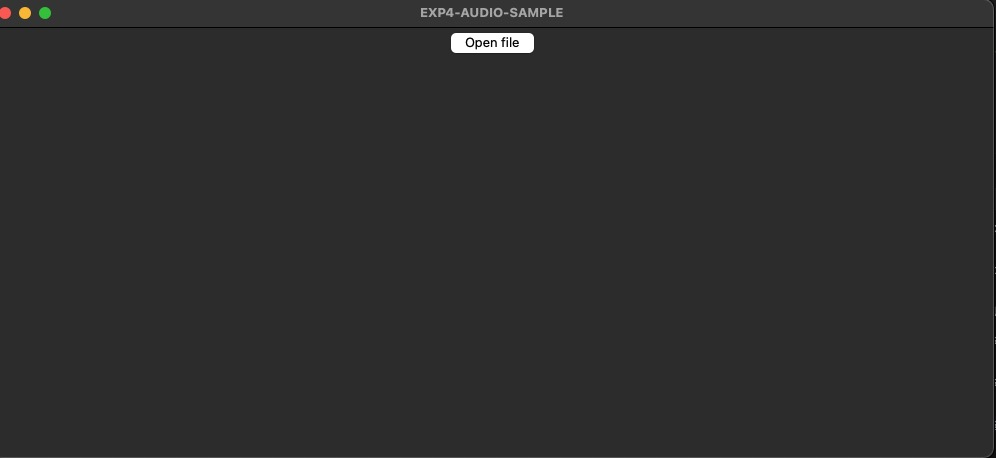
\includegraphics[width=120mm]{img/init.jpg}
  \caption{初期画面}
\end{figure}
\begin{figure}[H]
  \centering
  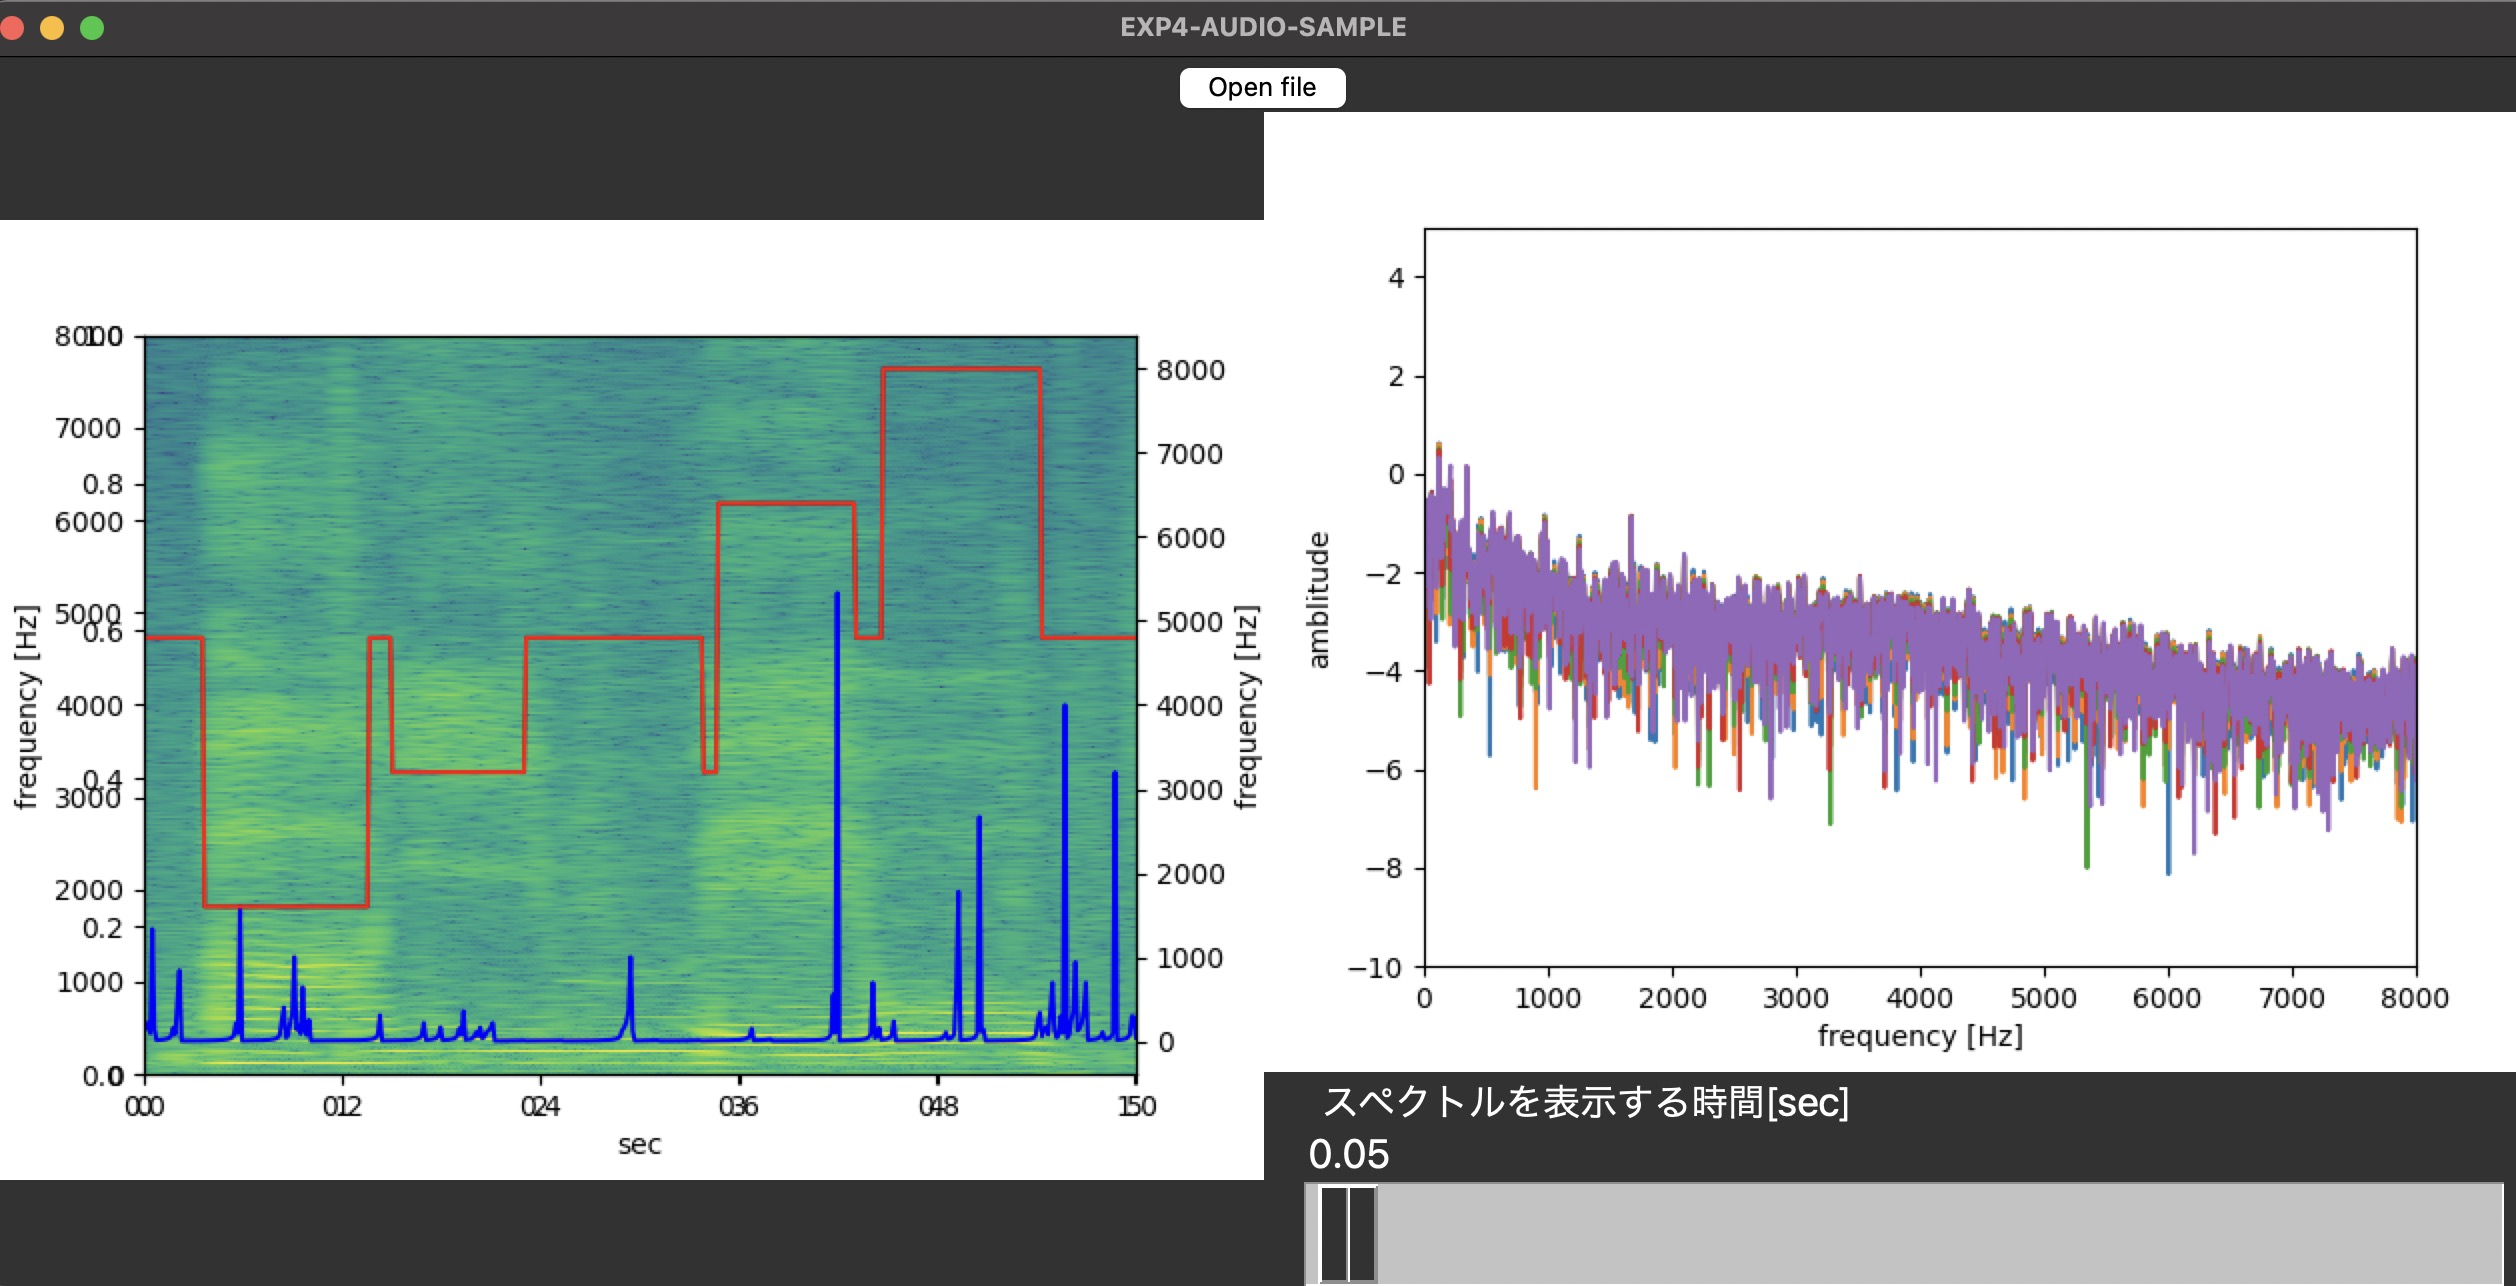
\includegraphics[width=120mm]{img/app2.jpg}
  \caption{アプリのホーム画面}
\end{figure}
\clearpage
\section{プログラムの説明}
\subsection{プログラムの構成}
今回の課題1では,以下のような関数構成となっている.
\begin{verbatim}
(main)
├─openfile
  ├─ calc
  │  ├── is_peak
  │  └── vowel_recognition
  ├─  draw_data
  └─ _draw_spectrum
\end{verbatim}

\subsection{各関数の説明}
\subsection{main}.
GUIアプリケーションのメイン関数.tkinterの初期配置や,ボタンを押した際呼び出される関数を定義している.
実際には定義していないが,便宜上main関数として扱っているものである.
\paragraph*{ソースコード}
\begin{lstlisting}[caption=main関数,label=openfile]

def open_file(event):
  (略)

# Tkinterを初期化
root = tkinter.Tk()
root.wm_title("EXP4-AUDIO-SAMPLE")

# ファイルを開く
open_file_button = tkinter.Button(root, text='Open file')
open_file_button.pack(side=tkinter.TOP)
open_file_button.bind('<Button-1>', open_file)

# # 再生ボタン (生やす予定が実装が間に合わなかったものである)
# play_music_button = tkinter.Button(root, text='Play')
# play_music_button.pack(side=tkinter.END)
# play_music_button.bind('<Button-1>', play_music)

tkinter.mainloop()
\end{lstlisting}
\subsubsection{openfile}
openfile関数は,tkinterのfiledialogを用いて音響信号ファイルを選択し,それを元に
音響信号のスペクトログラム,基本周波数,母音推定を行う.関数である,内部には
is\_peak関数,draw\_spectrum関数が存在する.
\paragraph*{ソースコード}
\begin{lstlisting}[caption=openfile関数,label=openfile]
def open_file(event):
  # tkinterで読み込む
  fTyp = [("wav file", "*.wav")]
  iDir = os.path.abspath(os.path.dirname(__file__))
  global input_file
  input_file = tkinter.filedialog.askopenfilename(filetypes=fTyp, initialdir=iDir)
  # 音声ファイルを読み込む
  x, _ = librosa.load(input_file, sr=SR)

  # ファイルサイズ(秒)
  duration = len(x) / SR

  # ハミング窓
  hamming_window = np.hamming(size_frame)

  def calc(x):
    (略)
  def _draw_data(spectrogram, hz_list):
    (略)
  def _draw_spectrum(v):
    (略)
  # スペクトルを表示する領域を確保
  # ax2, canvs2 を使って上記のコールバック関数でグラフを描画する
  fig2, ax2 = plt.subplots()
  canvas2 = FigureCanvasTkAgg(fig2, master=frame2)
  canvas2.get_tk_widget().pack(side="top")    # "top"は上部方向にウィジェットを積むことを意味する

  # スライドバーを作成
  scale = tkinter.Scale(
      command=_draw_spectrum,        # ここにコールバック関数を指定
      master=frame2,                # 表示するフレーム
      from_=0,                    # 最小値
      to=duration,                # 最大値
      resolution=size_shift/SR,    # 刻み幅
      label=u'スペクトルを表示する時間[sec]',
      orient=tkinter.HORIZONTAL,    # 横方向にスライド
      length=600,                    # 横サイズ
      width=50,                    # 縦サイズ
      font=("", 20)                # フォントサイズは20pxに設定
  )
  scale.pack(side="top")
\end{lstlisting}
\subsubsection{is\_peak}
is\_peak関数は,基本周波数の推定を行う関数である.
基本周波数の推定は,スペクトルのピークを求めることで行うことができるので(cf. 演習11),
これを用いてシフト幅を変えながら基本周波数を推定する.
\paragraph*{ソースコード}
\begin{lstlisting}[caption=is\_peak関数,label=openfile]
def is_peak(a, index):
if index == 0 or index == len(a)-1:
    return False
if a[index-1] < a[index] and a[index] > a[index+1]:
    return True
else:
    return False

\end{lstlisting}
\subsubsection{calc}
calc関数は,openfile関数内で呼び出される関数である.
calc関数は,openfile関数内で読み込んだ音響信号を元にスペクトログラム,基本周波数,母音推定を行う.
引数にはlibrosaで読み込んだ音響信号xを与え,,返り値にスペクトログラム,基本周波数,母音推定の結果のデータを返す.
\paragraph*{ソースコード}
\begin{lstlisting}[caption=calc関数,label=openfile]
def is_peak(a, index)
(略)

# スペクトログラムを保存するlist
  spectrogram = []
  hz_list = []
  pred = []
  autocorr = np.correlate(x, x, 'full')

  # 不要な前半を捨てる
  autocorr = autocorr[len(autocorr) // 2:] 
  # フレーム毎にスペクトルを計算
  for i in np.arange(0, len(x)-size_frame, size_shift):
      
      # 該当フレームのデータを取得
      start_idx = int(i)    # arangeのインデクスはfloatなのでintに変換
      end_idx = start_idx+size_frame
      x_frame = x[start_idx: end_idx]

      # スペクトル
      fft_spec = np.fft.rfft(x_frame * hamming_window)
      fft_log_abs_spec = np.log(np.abs(fft_spec))
      spectrogram.append(fft_log_abs_spec)
      
      # 基本周波数
      # 区間ごとの自己相関を取得
      autocorr_interval = autocorr[start_idx:end_idx]
          # ピークのインデックスを抽出する
      peakindices = [i for i in range(len(autocorr_interval)) if is_peak(autocorr_interval, i)]
          # インデックス0 がピークに含まれていれば捨てる
      peakindices = [i for i in peakindices if i != 0]
          # 自己相関が最大となるインデックスを得る
      max_peak_index = max(peakindices, key=lambda index: autocorr_interval[index])
      # max_peak_index_interval = np.argmax(autocorr_interval)
      # 区間ごとの周波数を計算して出力
      freq_interval = SR / max_peak_index
      hz_list.append(freq_interval)
      
      # 母音の判定
      cep = np.real(np.fft.rfft(fft_log_abs_spec))
      cep = cep[:13]
      likelihood_a = calc_likelihood(cep, mu_a, var_a)
      likelihood_i = calc_likelihood(cep, mu_i, var_i)
      likelihood_u = calc_likelihood(cep, mu_u, var_u)
      likelihood_e = calc_likelihood(cep, mu_e, var_e)
      likelihood_o = calc_likelihood(cep, mu_o, var_o)
      likelihood = [likelihood_a, likelihood_i, likelihood_u, likelihood_e, likelihood_o]
      pred.append((likelihood.index(max(likelihood))+ 1)* SR / 10)
  return spectrogram, hz_list, pred
\end{lstlisting}
\subsubsection{draw\_data}
draw\_data関数は,calc関数で得られたスペクトログラムをGUIアプリケーションの左側に表示する関数である.
引数としてスペクトログラムと基本周波数,母音推定の結果のリストのデータを与え,返り値は持たない.
\paragraph*{ソースコード}
\begin{lstlisting}[caption=draw\_data関数,label=openfile]
def _draw_data(spectrogram, hz_list, pred):
  # まずはスペクトログラムを描画
  fig, ax = plt.subplots()
  canvas = FigureCanvasTkAgg(fig, master=frame1)    # masterに対象とするframeを指定
  ax1 = fig.add_subplot(111)
  ax1.set_xlabel('sec')
  ax1.set_ylabel('frequency [Hz]')
  ax1.imshow(
      np.flipud(np.array(spectrogram).T),
      extent=[0, duration, 0, 8000],
      aspect='auto',
      interpolation='nearest'
  )
  # 続いて右側のy軸を追加して,音量を重ねて描画
  ax3 = ax1.twinx()
  ax3.set_ylabel('frequency [Hz]')
  x_data = np.linspace(0, duration, len(hz_list))
  ax3.plot(x_data, hz_list, c='b')
  ax3.plot(x_data, pred, c='r')
  canvas.get_tk_widget().pack(side="left")    # 最後にFrameに追加する処理
\end{lstlisting}
\subsubsection{draw\_spectrum}
draw\_spectrum関数は,指定された位置の音響信号のスペクトルをGUIアプリケーションの右側に表示する関数である.
引数としてスライダーの値を与え,返り値は持たない.
\paragraph*{ソースコード}
\begin{lstlisting}[caption=\_draw\_spectrum関数,label=openfile]
def _draw_spectrum(v):

  # スライドバーの値からスペクトルのインデクスおよびそのスペクトルを取得
  index = int((len(spectrogram)-1) * (float(v) / duration))
  spectrum = spectrogram[index]

  # 直前のスペクトル描画を削除し,新たなスペクトルを描画
  plt.cla()
  x_data = np.fft.rfftfreq(size_frame, d=1/SR)
  ax2.plot(x_data, spectrum)
  ax2.set_ylim(-10, 5)
  ax2.set_xlim(0, SR/2)
  ax2.set_ylabel('amblitude')
  ax2.set_xlabel('frequency [Hz]')
  canvas2.draw()

\end{lstlisting}

\section{工夫した点,今後の展望}
既存のコードを参考にしながら,できるだけ拡張性を意識したコードにした.
具体的には,関数配置を見直し,関数の再利用性を高めた.
tkinterでのUI追加を行う場合,これまでの記法を流用して書きやすいようになっている.
また,サンプルコードを参考にしながら,スライダーを作成しその位置に対応するスペクトルを表示する機能もできた.
今後余裕があれば,再生ボタンを追加し再生しながらスペクトルを出したり,波形を出したりできるようにしたい.

付録: 全ソースコードはこちら→\url{https://github.com/Mntisgod/isle4-audio}.\\

\end{document}


